\chapter{\texorpdfstring{\(SU(5)\)}{SU(5)} 多重态、轻夸克规范玻色子与质子衰变}

\lectureoverview{当标准模型群被嵌入 \(SU(5)\) 中时，大统一就变得具体了。为了看清这一陈述的含义，我们首先建立必要的表示论：定义表示 \(N\)、其共轭 \(\overline N\)、张量积、对称与反对称张量以及伴随表示。一个标准模型代便落入出乎意料地经济的组合 \(\overline{\mathbf 5}\oplus\mathbf{10}\) 中。使这一安排显得优美的同一种对称性，也要求存在将夸克转变为轻子的带色规范玻色子。它们的交换允许质子衰变，从而把统一能标推向 \(10^{15}\)--\(10^{16}\,\mathrm{GeV}\)。跑动的规范耦合指向一个相近的能标，而超对称在最后重新出现，因为它使三者的数值交汇显著更加精确。}

\section{为什么要从群表示开始？}

已有许多被提出的大统一理论。我们不去综述它们，而是剖析一个例子并提出三个问题：它为什么能成立，它要求哪些新粒子，以及实验在何处使它陷入危险。这个群是 \(SU(5)\)，其定义性的结构特征是嵌入
\begin{equation}
SU(3)_c\times SU(2)_L\times U(1)_Y
\subset SU(5).
\label{eq:l10-sm-embedding}
\end{equation}
这里 \(SU(3)_c\) 作用于色，\(SU(2)_L\) 作用于弱同位旋，\(U(1)_Y\) 作用于超荷。

超对称并不是这一构造的前提。超对称与大统一在逻辑上都不蕴含对方。它们在本讲中的联系是数值性的：当把超伴侣谱纳入重整化群计算时，三个规范耦合更精确地趋近一个共同值。

被某种对称性相互混合的粒子构成该对称群的表示。因此，对统一的粒子多重态进行分类首先需要一点表示论。

\subsection{熟悉的 \texorpdfstring{\(SU(2)\)}{SU(2)} 例子}

与普通角动量相联系的 \(SU(2)\) 与三维空间的旋转密切相关。更确切地说，\(SU(2)\) 是 \(SO(3)\) 的双重覆盖。其不可约表示由
\begin{equation}
j=0,\frac12,1,\frac32,\ldots,
\qquad
\dim(j)=2j+1.
\label{eq:l10-su2-spins}
\end{equation}
标记。因此标量是单态，自旋 \(\tfrac12\) 粒子是双重态，自旋为一的粒子是三重态。弱群 \(SU(2)_L\) 是不同的物理对称性，尽管其抽象群论相同。

\section{定义表示及其共轭}

对于 \(SU(N)\)，定义表示是复 \(N\) 分量列向量的空间，
\begin{equation}
\psi=
\begin{pmatrix}
\psi_1\\
\psi_2\\
\vdots\\
\psi_N
\end{pmatrix},
\qquad
\psi'_i=U_i{}^j\psi_j,
\qquad
U\in SU(N).
\label{eq:l10-defining}
\end{equation}
它被称为定义表示，或简称为 \(\mathbf N\)。矩阵 \(U\) 是 \(N\times N\)，它们所作用的向量空间维数为 \(N\)。

复共轭给出另一个 \(N\) 维表示，
\begin{equation}
\psi_i^*\longmapsto U_i{}^{j*}\psi_j^*,
\label{eq:l10-conjugate}
\end{equation}
记作 \(\overline{\mathbf N}\)。对于 \(N>2\)，定义表示与共轭表示不等价。人们可以交换哪一个被称为粒子表示、哪一个被称为反粒子表示，但一旦选定一种约定，就必须固定不变。

\begin{classroomqa}
\audiencequestion{\(SU(N)\) 中的 \(N\) 是否取决于 \(N\) 是偶数还是奇数，它指的是矩阵吗？\lecturetimestamp{00:07:33}}
\lecturerresponse{这里没有偶--奇的限制。\(N\) 是定义矩阵的大小，也是其定义表示的维数。\(\mathbf N\) 和 \(\overline{\mathbf N}\) 都具有该维数。}
\end{classroomqa}

反粒子的反粒子就是原来的粒子。这就是为什么交换 \(\mathbf N\) 与 \(\overline{\mathbf N}\) 的名称改变的是约定而非物理。

\section{张量积与不可约性}

假设一个物体可以占据 \(N\) 个内部态，而另一个物体可以独立地占据同样数目的内部态。忽略位置、动量、自旋以及除这个 \(SU(N)\) 标记以外的每一个量子数，这一对物体有
\begin{equation}
N\times N=N^2
\label{eq:l10-product-count}
\end{equation}
个态。如果第一个物体处于态 \(\psi_i\)，第二个处于态 \(\phi_j\)，它们的乘积可以写作
\begin{equation}
\Psi_{ij}=\psi_i\phi_j,
\qquad
\Psi'_{ij}=U_i{}^kU_j{}^\ell\Psi_{k\ell}.
\label{eq:l10-tensor-transform}
\end{equation}
这就是张量积 \(\mathbf N\otimes\mathbf N\)。

\begin{classroomqa}
\audiencequestion{为什么答案是 \(N^2\) 而不是 \(N^2-1\)，允许两个粒子具有相同的内部标记是否违反不相容原理？\lecturetimestamp{00:10:22}}
\lecturerresponse{这里两个位置是可区分的：一个物体固定在一个位置，另一个固定在另一个位置。泡利原理约束的是包括位置在内的完整量子态。它并不会去掉这些 \(N^2\) 个内部标记组合中的任何一个。数目 \(N^2-1\) 稍后将在另一个乘积中由无迹条件产生。}
\end{classroomqa}

\(N^2\)维乘积表示一般是可约的。当一个表示包含群映射到自身的真子空间时，它就是可约的。不变子空间可以被分离出来并作为更小的表示来处理；如果不存在这样的真子空间，则该表示是不可约的。

\subsection{对称张量与反对称张量}

每个二指标张量都唯一地分解为
\begin{align}
\Psi_{ij}
&=\Psi^{(S)}_{ij}+\Psi^{(A)}_{ij},\\
\Psi^{(S)}_{ij}
&=\frac12(\Psi_{ij}+\Psi_{ji}),\\
\Psi^{(A)}_{ij}
&=\frac12(\Psi_{ij}-\Psi_{ji}).
\label{eq:l10-sym-anti}
\end{align}
这两部分满足
\begin{equation}
\Psi^{(S)}_{ij}=\Psi^{(S)}_{ji},
\qquad
\Psi^{(A)}_{ij}=-\Psi^{(A)}_{ji}.
\end{equation}
式~\eqref{eq:l10-tensor-transform}保持每个条件不变，因此群变换绝不会混合对称与反对称部分。

\editorialnote{讲义把一般计数留作练习。对称与反对称的维数分别为\(N(N+1)/2\)和\(N(N-1)/2\)，它们的和为\(N^2\)。}

\begin{figure}[htbp]
\centering
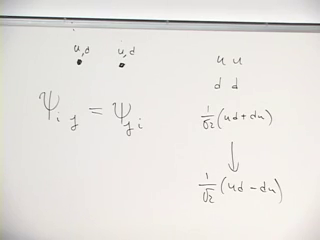
\includegraphics[width=0.78\textwidth]{lecture_10_figure_02.png}
\lectureframe{00:17:57.500}
\caption{两个自旋\(\tfrac12\)态所构成的完整基底分解：三个对称态和一个反对称态。}
\label{fig:l10-spin-decomposition}
\end{figure}

对于\(SU(2)\)的定义二重态，
\begin{equation}
\mathbf2\otimes\mathbf2=\mathbf3_S\oplus\mathbf1_A.
\label{eq:l10-two-two}
\end{equation}
把两个基态写为\(u\)和\(d\)，对称三重态为
\begin{align}
\ket{1,1}&=\ket{uu},\\
\ket{1,0}&=\frac{1}{\sqrt2}\bigl(\ket{ud}+\ket{du}\bigr),\\
\ket{1,-1}&=\ket{dd},
\end{align}
而反对称单态为
\begin{equation}
\ket{0,0}
=\frac{1}{\sqrt2}\bigl(\ket{ud}-\ket{du}\bigr).
\end{equation}
这就是熟悉的两个自旋\(\tfrac12\)角动量的相加：四个原始态重新组合成自旋一和自旋零。

\section{粒子与反粒子：伴随表示}

现在把定义表示与其共轭表示组合起来。乘积仍然有\(N^2\)个分量，但它按矩阵变换：
\begin{equation}
M_i{}^j\in\mathbf N\otimes\overline{\mathbf N},
\qquad
M\longmapsto U M U^\dagger.
\label{eq:l10-matrix-transform}
\end{equation}
与\(\mathbf N\otimes\mathbf N\)不同，一个基本指标和一个反基本指标之间没有有意义的交换对称性。自然的分解反而是
\begin{equation}
M
=
\frac{\operatorname{tr}M}{N}\,\mathbf1_N
+
\left(M-\frac{\operatorname{tr}M}{N}\,\mathbf1_N\right).
\label{eq:l10-trace-split}
\end{equation}
第一项是单态，无迹部分则是伴随表示：
\begin{equation}
\mathbf N\otimes\overline{\mathbf N}
=\mathbf1\oplus\mathbf{Adj},
\qquad
\dim\mathbf{Adj}=N^2-1.
\label{eq:l10-adjoint}
\end{equation}

\begin{figure}[htbp]
\centering
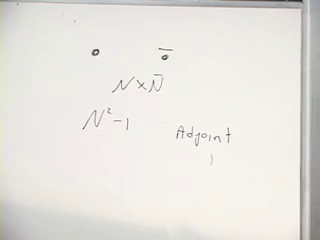
\includegraphics[width=0.67\textwidth]{lecture_10_figure_04.png}
\lectureframe{00:23:47.500}
\caption{关于\(\mathbf N\otimes\overline{\mathbf N}\)的黑板结论：其无迹的\(N^2-1\)个分量构成伴随表示。}
\label{fig:l10-adjoint}
\end{figure}

对于\(SU(3)\)，这给出熟悉的八重态，
\begin{equation}
\mathbf3\otimes\overline{\mathbf3}
=\mathbf8\oplus\mathbf1,
\end{equation}
而八个胶子在伴随表示中变换。对于\(SU(2)\)，伴随表示的维数为三，并像自旋一那样变换。

\section{一个标准模型代}

观测到有三代，但\(SU(5)\)对每一代分别重复同样的构造。它并不解释为什么有三份拷贝。因此我们集中讨论第一代。

所有场都将写成左手Weyl场。右手费米子由其左手电荷共轭场表示：
\begin{equation}
u^c_L,\qquad d^c_L,\qquad e^c_L.
\label{eq:l10-left-handed-bookkeeping}
\end{equation}
上标\(c\)表示电荷共轭；例如，\(d^c_L\)是电荷为\(+\tfrac13\)的左手反下夸克场。

在标准的\(SU(5)\)记号中，十五个左手场中有五个放入
\begin{equation}
\overline{\mathbf5}
=
\begin{pmatrix}
\nu_{eL}\\
e_L\\
d^c_{rL}\\
d^c_{gL}\\
d^c_{bL}
\end{pmatrix}.
\label{eq:l10-fivebar}
\end{equation}
顺序被选为先是弱二维块，随后是色三维块。弱变换混合前两个分量，色变换混合最后三个分量，而非对角\(SU(5)\)生成元连接这两个块。

\editorialnote{讲义把式~\eqref{eq:l10-fivebar}中的列称为\(\mathbf5\)，后来把反对称多重态称为\(\overline{\mathbf{10}}\)。这是整体共轭的约定。我们采用现代标准的\(\overline{\mathbf5}\oplus\mathbf{10}\)；对每个表示取共轭即可重现讲义的标签，而不改变其物理。}

完整的最小第一代清单是
\begin{equation}
\begin{gathered}
\underbrace{Q_L=(u_L,d_L)}_{6}
\oplus
\underbrace{L_L=(\nu_{eL},e_L)}_{2},\\
\underbrace{u^c_L}_{3}
\oplus
\underbrace{d^c_L}_{3}
\oplus
\underbrace{e^c_L}_{1},\\
6+2+3+3+1=15.
\end{gathered}
\label{eq:l10-fifteen}
\end{equation}
最小标准模型没有独立的\(\nu^c_L\)，因此它不给出可重整化的中微子质量。中微子振荡表明这一最小陈述是不完整的：自然界具有小的非零中微子质量，因此需要扩展。

\begin{classroomqa}
\audiencequestion{当费米子质量把左手态变为右手态时，它是否也把粒子变成其反粒子？\lecturetimestamp{00:34:00}}
\lecturerresponse{不。电子质量把左手电子连接到具有相同电荷的右手电子。在全左手记号中，第二个场由\(e^c_L\)表示，但四分量粒子仍然是电子。只有中性场才能具有把粒子与反粒子等同起来的Majorana质量。}
\end{classroomqa}

\section{五重态中可见的规范玻色子}

规范对称性的每个生成元都有一个相应的规范场。在式~\eqref{eq:l10-fivebar}中，熟悉的跃迁已经可以辨认出来：
\begin{itemize}
\item 弱规范场在\(\nu_{eL}\)和\(e_L\)之间作用；
\item 胶子在\(d^c_L\)的三种颜色之间作用；
\item 中性生成元对角作用；
\item 新的非对角生成元把一个轻子分量转换为一个带色分量，或反之。
\end{itemize}

胶子可以被描绘为携带夸克--反夸克色量子数。讲义使用通常的世界线助记法：沿一条出射反夸克的世界线反向穿过发射顶点，它看起来就像一条正向运行的夸克。因此，发射出的场携带一个夸克--反夸克对的量子数。用表示论的语言来说，这恰好是\(\mathbf3\otimes\overline{\mathbf3}\)的无迹部分。

对于\(SU(5)\)，
\begin{equation}
\dim\mathbf{Adj}_{SU(5)}=5^2-1=24.
\end{equation}
这些规范场在标准模型子群下的分解为
\begin{equation}
\mathbf{24}
=
(\mathbf8,\mathbf1)_0
\oplus(\mathbf1,\mathbf3)_0
\oplus(\mathbf1,\mathbf1)_0
\oplus(\mathbf3,\mathbf2)_{-5/6}
\oplus(\overline{\mathbf3},\mathbf2)_{5/6},
\label{eq:l10-adjoint-sm}
\end{equation}
其中有序对表示\(SU(3)_c\times SU(2)_L\)，下标为超荷。

\editorialnote{方程~\eqref{eq:l10-adjoint-sm}明确给出了讲义中所画的块状结构。前三项包含熟悉的色规范场和电弱规范场。最后两项是十二个实自由度，习惯上称为\(X\)和\(Y\)玻色子。}

\begin{figure}[htbp]
\centering
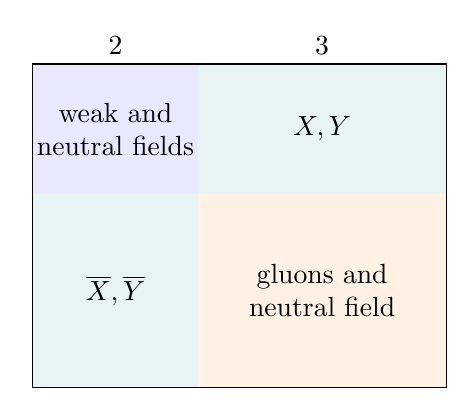
\begin{tikzpicture}[x=1.05cm,y=0.82cm]
  \draw[thick] (0,0) rectangle (5,5);
  \draw[thick] (2,0) -- (2,5);
  \draw[thick] (0,3) -- (5,3);
  \fill[blue!9] (0,3) rectangle (2,5);
  \fill[orange!10] (2,0) rectangle (5,3);
  \fill[teal!9] (2,3) rectangle (5,5);
  \fill[teal!9] (0,0) rectangle (2,3);
  \node[align=center] at (1,4) {weak and\\neutral fields};
  \node[align=center] at (3.5,1.5) {gluons and\\neutral field};
  \node[align=center] at (3.5,4) {\(X,Y\)};
  \node[align=center] at (1,1.5) {\(\overline X,\overline Y\)};
  \node[above] at (1,5) {\(2\)};
  \node[above] at (3.5,5) {\(3\)};
\end{tikzpicture}
\caption{\(SU(5)\)规范场的\(2\oplus3\)块状结构。非对角块连接轻子与带色场。}
\label{fig:l10-gauge-blocks}
\end{figure}

在\(Q=T_3+Y\)下，式~\eqref{eq:l10-adjoint-sm}中的带色弱二重态具有电荷\(-\tfrac13\)和\(-\tfrac43\)；其共轭具有\(+\tfrac13\)和\(+\tfrac43\)。讲义称这些粒子为\(X\)和\(Y\)，但明确拒绝确定哪个名称对应哪个电荷。跃迁和电荷才是不变的内容。

\begin{classroomqa}
\audiencequestion{每种新的\(X\)或\(Y\)规范玻色子都有三个版本吗？\lecturetimestamp{00:41:28}}
\lecturerresponse{是的。一个跃迁将带色夸克条目连接到无色轻子条目，因此交换的玻色子必须携带缺失的色。\(X/Y\)场构成色三重态，并且可以发射或吸收胶子。}
\end{classroomqa}

带色粒子不会作为孤立的渐近态被观测到。新的规范玻色子必须衰变或强子化为色中性组合，正如夸克那样。

\section{为什么该多重态包含反下夸克}

\(SU(N)\)的生成元是无迹厄米矩阵。为了看出与“特殊”一词的联系，将无穷小群元素写为
\begin{equation}
U(\epsilon)=e^{i\epsilon T}.
\end{equation}
幺正性给出\(T^\dagger=T\)，而
\begin{equation}
1=\det U=e^{i\epsilon\operatorname{tr}T}
\end{equation}
对任意\(\epsilon\)给出
\begin{equation}
\operatorname{tr}T=0.
\label{eq:l10-traceless-generator}
\end{equation}

电荷是生成元的线性组合。在式~\eqref{eq:l10-fivebar}的物质列上，它作用为
\begin{equation}
Q_{\overline5}
=
\operatorname{diag}
\left(0,-1,\frac13,\frac13,\frac13\right),
\qquad
\operatorname{tr}Q_{\overline5}=0.
\label{eq:l10-charge-fivebar}
\end{equation}
因此
\begin{equation}
0-1+3\left(\frac13\right)=0.
\end{equation}
若将反下夸克场替换为下夸克场，则会得到
\begin{equation}
0-1+3\left(-\frac13\right)=-2,
\end{equation}
这不能是\(SU(5)\)生成元的迹。因此，看似奇怪的反下夸克分配是由群结构强制的。

\section{剩余的十个费米子}

另外十个场来自一个反对称双指标张量。在标准约定下，这是
\begin{equation}
\mathbf5\otimes\mathbf5
=\mathbf{15}_S\oplus\mathbf{10}_A.
\label{eq:l10-five-five}
\end{equation}
的反对称部分。讲义通过暂时写出共轭量子数
\begin{equation}
\chi=
\begin{pmatrix}
\nu^c\\
e^c\\
d_r\\
d_g\\
d_b
\end{pmatrix}.
\label{eq:l10-aux-five}
\end{equation}
来构造它。这是一种用于张量表示直积的记账手段，而不是声称存在第二个由复合粒子组成的物理五重态。

令
\begin{equation}
\Psi^{ij}=-\Psi^{ji},
\qquad
i,j=1,\ldots,5.
\label{eq:l10-antisym-ten}
\end{equation}
所有对角元都为零，下三角由上三角确定。因此
\begin{equation}
\dim\mathbf{10}
=\binom52
=\frac{5\cdot4}{2}
=10.
\label{eq:l10-ten-count}
\end{equation}

一个条目的电荷是式~\eqref{eq:l10-aux-five}中行电荷与列电荷之和。这立即给出弱--弱槽位中的\(e^c\)、弱--色块中的下夸克和上夸克，以及色--色块中的反上夸克场。

\begin{classroomqa}
\audiencequestion{当正电子和下夸克标签组合时，所得条目应该是\(X\)玻色子吗？\lecturetimestamp{00:53:08}}
\lecturerresponse{不是。在这个阶段，我们构造的是费米子表示，而不是规范玻色子伴随表示。电荷相加为\(1-\tfrac13=\tfrac23\)，因此该条目具有上夸克的量子数。}
\end{classroomqa}

一种自洽的色符号选择是
\begin{equation}
\Psi^{ij}=
\begin{pmatrix}
0 & e^c & d_r & d_g & d_b\\
-e^c & 0 & u_r & u_g & u_b\\
-d_r & -u_r & 0 & u_b^c & -u_g^c\\
-d_g & -u_g & -u_b^c & 0 & u_r^c\\
-d_b & -u_b & u_g^c & -u_r^c & 0
\end{pmatrix}.
\label{eq:l10-ten-matrix}
\end{equation}
改变场相位会改变一些显示出来的符号，但不会改变表示或粒子内容。

\begin{figure}[htbp]
\centering
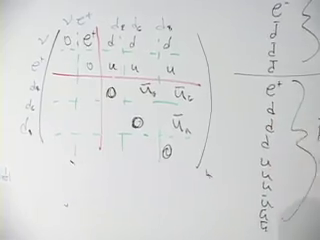
\includegraphics[width=0.83\textwidth]{lecture_10_figure_05.png}
\lectureframe{00:59:17.500}
\caption{在课堂上检查了条目和色标签之后，无阻碍的\(2\oplus3\)反对称物质矩阵。}
\label{fig:l10-ten-board}
\end{figure}

\begin{classroomqa}
\audiencequestion{十维表示必须写成矩阵，还是可以写成一列？\lecturetimestamp{00:56:24}}
\lecturerresponse{两者都可以。人们可以把十个独立分量列成一列，但反对称\(5\times5\)矩阵展示了\(SU(5)\)如何作用于它的两个指标，因此信息量大得多。}
\end{classroomqa}

\begin{classroomqa}
\audiencequestion{在色--色块中，标记为\(u\)的条目实际上是否应为反上夸克场？\lecturetimestamp{00:57:51}}
\lecturerresponse{是的。黑板上的标记更正为\(u^c\)，即左手反上夸克场。两个下型基态电荷之和为\(-\tfrac23\)，这正是反上夸克的电荷。}
\end{classroomqa}

\begin{classroomqa}
\audiencequestion{若干矩阵元中省略了色。它们仍然守恒吗？\lecturetimestamp{00:58:05}}
\lecturerresponse{是的。三个色位分别是红、绿、蓝。省略标记只是为了减少杂乱。}
\end{classroomqa}

一对反对称的色基础表示变换为反色：
\begin{equation}
\wedge^2\mathbf3\simeq\overline{\mathbf3},
\qquad
(rg,rb,gb)\sim(\overline b,-\overline g,\overline r).
\label{eq:l10-anticolor}
\end{equation}
这就是为什么色--色块中的三个独立条目恰好构成反上夸克色三重态。

一个世代现在被组织为
\begin{equation}
\overline{\mathbf5}\oplus\mathbf{10}.
\label{eq:l10-family}
\end{equation}
引人注目的是，\(u_L\)和\(u^c_L\)出现在同一个不可约多重态中，而\(d_L\)和\(d^c_L\)，或\(e_L\)和\(e^c_L\)，则位于不同的多重态中。

\begin{classroomqa}
\audiencequestion{如果规范变换只在每个表示内部作用，那么质量如何能连接位于五重态反表示和十重态中的场？\lecturetimestamp{01:00:40}}
\lecturerresponse{规范玻色子不会将一个不可约物质表示旋转为另一个。希格斯场和汤川耦合可以连接不同的表示，同时形成一个整体的\(SU(5)\)不变相互作用；在希格斯场获得期望值之后，这些相互作用产生质量。}
\end{classroomqa}

\section{规范玻色子作为移位作用}

在表示被组装起来之后，规范玻色子的作用可以读作其条目之间的移位。中性玻色子可以使标记保持不变，弱玻色子在弱位之间移动，胶子在色位之间移动，而\(X/Y\)玻色子在弱位与色位之间移动。带电规范玻色子有反粒子，因此每种移位都有一个逆过程。

对于反对称张量，无穷小变换作用于任一指标：
\begin{equation}
\delta\Psi^{ij}
=
i\epsilon
\left(
T^i{}_k\Psi^{kj}
+
T^j{}_k\Psi^{ik}
\right).
\label{eq:l10-two-index-action}
\end{equation}
在矩阵图像中，第一项垂直移动，第二项水平移动。用来构建张量的组分标记只是一种助记手段；式~\eqref{eq:l10-two-index-action}才是精确的群论陈述。

弱移位将\(d\)变为\(u\)，这是中子{\proseunicodefont β}衰变背后的夸克层次过程。色移位改变红、绿、蓝而不改变味。非对角移位则带来新东西：
\begin{equation}
\begin{aligned}
d^c&\longleftrightarrow e,
& d^c&\longleftrightarrow\nu,\\
d&\longleftrightarrow u^c,
& u&\longleftrightarrow e^c,
\end{aligned}
\label{eq:l10-leptoquark-shifts}
\end{equation}
其中相应的\(X/Y\)场携带电荷和色差。

\begin{classroomqa}
\audiencequestion{第四与第五个位之间的移位代表什么？从第一个位到第四个位的移位又如何？\lecturetimestamp{01:10:36}}
\lecturerresponse{第四--第五移位将一种色变为另一种色，是胶子跃迁。第一--第四移位跨越弱块与色块，是新的\(X/Y\)跃迁之一。}
\end{classroomqa}

\begin{classroomqa}
\audiencequestion{反对称矩阵下半部分的一个条目能否被显式填出？\lecturetimestamp{01:11:23}}
\lecturerresponse{可以。每个下三角条目都是转置后的上三角条目的负值。填出一个就能使规则可见；全部填出并不会增加新的态。}
\end{classroomqa}

\section{危险的后果：质子衰变}

\(X/Y\)玻色子可以在一个顶点将夸克耦合到轻子，在另一个顶点耦合到两个夸克型场。在远小于其质量的动量下，积掉重玻色子给出如下示意形式的六维相互作用
\begin{equation}
\mathcal L_{\mathrm{eff}}
\sim
\frac{g_5^2}{M_X^2}\,(qq)(q\ell)
+\text{h.c.}
\label{eq:l10-effective-proton}
\end{equation}
它分别破坏重子数和轻子数，同时保持统一规范相互作用所要求的组合。

黑板上追踪一个下夸克和一个上夸克经过重玻色子交换的过程。下夸克变成正电子，上夸克变成反上夸克，第二个上夸克是旁观者：
\begin{equation}
uud
\longrightarrow
e^++u\overline u.
\label{eq:l10-quark-decay}
\end{equation}
初态是质子。\(u\overline u\)对可以强子化为中性{\proseunicodefont π}介子，给出
\begin{equation}
p\longrightarrow e^++\pi^0.
\label{eq:l10-proton-pion}
\end{equation}

\begin{figure}[htbp]
\centering
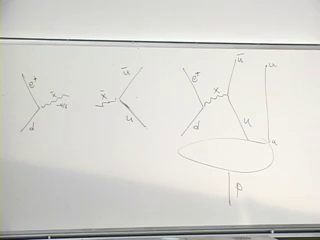
\includegraphics[width=0.82\textwidth]{lecture_10_figure_06.png}
\lectureframe{01:16:02.500}
\caption{质子内部重玻色子交换的完整黑板构建，旁观上夸克和正电子通道清晰可见。}
\label{fig:l10-proton-board}
\end{figure}

讲座还提到了\(p\to e^++\gamma\)，其中夸克--反夸克对通过电磁作用湮灭。相对于直接强子化，该通道带有额外的电磁压低。

这种可能性并非模型的可选装饰。一旦一个单群包含连接夸克与轻子的生成元，重子数破坏过程通常就是预期会出现的。如果它们发生在普通的弱或电磁时间尺度上，原子核、氢以及宏观物质都无法存续。

\section{为什么质子如此长寿？}

\begin{classroomqa}
\audiencequestion{产生\(X\)玻色的耦合，是否就是该群其余部分所用的同一个统一耦合？\lecturetimestamp{01:18:34}}
\lecturerresponse{在统一能标处，是的。一个简单的\(SU(5)\)规范理论只有一个规范耦合\(g_5\)。低能下的强、弱和超荷耦合之所以不同，是因为在统一对称性破缺之后，它们各自以不同的方式跑动。}
\end{classroomqa}

不能在不放弃统一结构的情况下把耦合选得极其小。可用的压低来自重传播子：
\begin{equation}
\mathcal A
\sim
\frac{g_5^2}{M_X^2}.
\label{eq:l10-amplitude}
\end{equation}
将振幅平方得到\(g_5^4/M_X^4\)。量纲分析和质子矩阵元补全了衰变率的估计：
\begin{equation}
\Gamma_p
\sim
C_{\mathrm{had}}\,
\frac{\alpha_5^2\,m_p^5}{M_X^4},
\qquad
\alpha_5=\frac{g_5^2}{4\pi},
\label{eq:l10-rate}
\end{equation}
其中\(C_{\mathrm{had}}\)包含群因子、重整化效应以及非微扰的强子矩阵元。

\editorialnote{本讲分离出本质性的\(g^4/M_X^4\)依赖关系，并指出质子质量因子被省略了。方程~\eqref{eq:l10-rate}恢复了所需的质量量纲，但并未声称这是精确的寿命计算。}

\begin{classroomqa}
\audiencequestion{在粗略的课堂估计中也许为\(10^{-8}\)量级的小因子\(g^4\)，是否已经足以使寿命变得足够长？\lecturetimestamp{01:25:13}}
\lecturerresponse{不。它有帮助，但微观强相互作用时间与质子寿命下限之间的差距跨越的 orders of magnitude 远不止这些。决定性的压低必须由重质量的四次方来提供。}
\end{classroomqa}

如果所有质量都在质子质量量级，那么自然的时间单位就近似为质子的光穿越时间：
\begin{equation}
t_p\sim\frac{1\ \mathrm{fm}}{c}\sim10^{-23}\ \mathrm{s}.
\label{eq:l10-proton-time}
\end{equation}
原初质子的存在本身就已经表明它们的寿命超过了宇宙年龄，但实验室搜寻远远走得更远。本讲将微观估计与当时引用的实验下限
\begin{equation}
\tau_p\gtrsim10^{33}\ \mathrm{yr}.
\label{eq:l10-lifetime-bound}
\end{equation}进行比较。

人们不必对单个质子观察那么久。如果寿命为\(10^{15}\)年，那么\(10^{15}\)个质子的样品每年大约会产生一个事件。更一般地，若在时间\(T\)内观测\(N_p\)个质子，则预期衰变数为
\begin{equation}
\langle n\rangle\simeq\frac{N_pT}{\tau_p}.
\label{eq:l10-event-count}
\end{equation}
一个包含大约\(10^{33}\)个质子的探测器是一个大罐子，而不是一个天文物体：质子本身的质量约为\(10^6\)千克。观测这样的样品，就把一个巨大的单个寿命转化为可测量的事件率，或转化为更强的下限。

将方程~\eqref{eq:l10-rate}与寿命约束结合起来，会把轻夸克规范玻色子的质量推向
\begin{equation}
M_X\sim10^{15}\text{--}10^{16}\ \mathrm{GeV},
\label{eq:l10-mx}
\end{equation}
其中\(10^{16}\,\mathrm{GeV}\)在本讲中被用作便于记忆的安全能标。这比普朗克能标低若干 orders of magnitude，因此并不自动与量子场论矛盾。

\section{破缺的\texorpdfstring{\(SU(5)\)}{SU(5)}与统一能标}

\(X/Y\)场与标准模型规范场共享一个\(SU(5)\)伴随多重态。严格未破缺的规范对称性不会允许其中某些成员的质量接近\(10^{16}\,\mathrm{GeV}\)，而光子和胶子却保持无质量。因此，该对称性必须自发破缺。

\begin{classroomqa}
\audiencequestion{如果\(SU(5)\)对称性未破缺，它的所有规范玻色子都会是无质量的吗？\lecturetimestamp{01:29:37}}
\lecturerresponse{是的，在所讨论的规范理论中如此。规范不变性禁止显式的共同质量。希格斯机制可以给与破缺生成元相联系的规范玻色子赋予质量，同时使未破缺子群的规范场保持无质量。}
\end{classroomqa}

电弱希格斯机制已经说明了这一模式：它把光子与\(W^\pm\)和\(Z\)区分开来。大统一需要一个单独的高能标序参量，它把弱的\(2\)块与色的\(3\)块区分开来，并使非对角\(X/Y\)场变得极其重。

与\(10^{16}\,\mathrm{GeV}\)相比，即使\(100\,\mathrm{GeV}\)的弱玻色子质量也可以忽略。在远高于重阈的地方，所有规范玻色子质量都可以忽略，完整的\(SU(5)\)对称性成为良好的近似。这就是统一能标的含义：并不是说低能世界明显地具有\(SU(5)\)，而是说能量足够高的过程变得对对称性破缺的质量劈裂不敏感。

\section{跑动耦合}

规范耦合以对数方式依赖于能标。定义
\begin{equation}
\alpha_i(\mu)=\frac{g_i^2(\mu)}{4\pi},
\end{equation}
单圈演化具有如下形式
\begin{equation}
\alpha_i^{-1}(\mu)
=
\alpha_i^{-1}(\mu_0)
-\frac{b_i}{2\pi}
\ln\!\left(\frac{\mu}{\mu_0}\right).
\label{eq:l10-running}
\end{equation}
系数\(b_i\)依赖于规范群，也依赖于每一个轻到足以在相关量子圈中循环的粒子。

\editorialnote{为了将超荷与\(SU(5)\)内部的非阿贝尔耦合进行比较，必须给\(g_1\)赋予传统的大统一归一化。这正是讲座中提到的数值群论因子的来源。}

在实验室能量下，三个耦合的倒数各不相同。按照讲座中的定性排序，\(1/\alpha_1\)最大，因为超荷最弱；\(1/\alpha_2\)次之；\(1/\alpha_3\)最小，因为强相互作用最强。在无法达到的能量处的曲线并非直接测量得到。它们是根据观测到的低能值、粒子谱以及决定贝塔函数的圈图计算出来的。在标准模型粒子内容下，当以\(\log\mu\)为横轴作图时，它们几乎成为直线。

\begin{figure}[htbp]
\centering
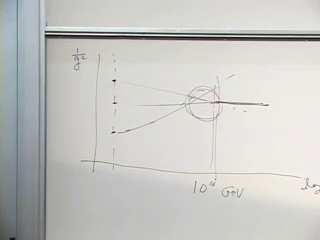
\includegraphics[width=0.74\textwidth]{lecture_10_figure_07.png}
\lectureframe{01:36:32.500}
\caption{黑板上画出的规范耦合倒数在\(10^{16}\,\mathrm{GeV}\)附近相互接近的图。圈出的区域标出了它们并不完美的交汇。}
\label{fig:l10-running-board}
\end{figure}

在大统一阈值以下，对称性破缺，轻粒子谱并不填满完整的简并\(SU(5)\)多重态，而且三个贝塔函数系数各不相同。因此，耦合以不同的速率跑动。在高能标下，人们要问它们是否达到一个共同值：
\begin{equation}
\alpha_1(M_{\mathrm{GUT}})
\stackrel{?}{=}
\alpha_2(M_{\mathrm{GUT}})
\stackrel{?}{=}
\alpha_3(M_{\mathrm{GUT}}).
\label{eq:l10-unification-condition}
\end{equation}

如果只有非超对称的标准模型谱，这些线在\(10^{15}\)--\(10^{16}\,\mathrm{GeV}\)附近相互接近，但偏差相当可观；讲座将这种符合程度描述为大约百分之十五。重要的巧合在于，这也正是质子稳定性所要求的能标。

\section{最后一个中子问题}

\begin{classroomqa}
\audiencequestion{如果把质子衰变图中的旁观上夸克换成下夸克，这会描述中子衰变吗？\(X\)玻色子会有影响吗？\lecturetimestamp{01:36:40}}
\lecturerresponse{这会定义一个诸如\(n\to e^++\pi^-\)的大统一中子道，但那并不是自由中子的熟悉衰变。普通中子贝塔衰变是\(n\to p+e^-+\overline\nu_e\)，并通过弱相互作用进行。如果质子--中子的质量顺序颠倒，贝塔稳定性也会颠倒，而慢得多的大统一道则可能仍然存在。}
\end{classroomqa}

这一区分把运动学与这种新相互作用分开。哪个核子发生贝塔衰变取决于质子--中子质量差；由\(X/Y\)交换引起的重子数破坏则是一种独立的、受到极大压低的机制。

\section{超对称性与更宏大的视角}

加入超对称伙伴谱会改变式~\eqref{eq:l10-running}中的贝塔函数系数。按照讲座的叙述，三个外推耦合随后以约百分之一的精度交汇。这并不能证明超对称或大统一，但它是这两种思想常被一起讨论的经验理由。

物质多重态还可以进一步统一。在
\begin{equation}
SO(10)\supset SU(5),
\end{equation}
之下，一个旋量表示分解为
\begin{equation}
\mathbf{16}
\longrightarrow
\mathbf{10}\oplus\overline{\mathbf5}\oplus\mathbf1.
\label{eq:l10-so10}
\end{equation}
这个单态自然被等同于左手反中微子，或者等价地，右手中微子的电荷共轭。因此，扩展代的所有十六个场都装入一个不可约的\(SO(10)\)多重态。

质子衰变实验继续检验这一思想：在未观测到事件时，就提高寿命下限。超对称大统一模型并不给出一个普适的质子寿命：额外重场以及依赖于超对称伙伴的算符可以在很宽的范围内改变主导道和衰变率。

\editorialnote{在超对称大统一中，色三重态希格斯交换除了这里讨论的六维规范玻色子算符之外，还能产生五维重子数破坏算符。它们的系数强烈依赖于重粒子谱、味结构以及超对称伙伴质量，这解释了讲座的警告：仅凭超对称并不能得出单一的寿命。}

持久的教训是一种张力，而不是一个定论。群论以惊人的经济性把夸克和轻子放在一起，跑动耦合暗示着一个共同的高能标，而超对称使这一数值暗示更加鲜明。同样的构造也预言了夸克向轻子的危险转化。因此，任何成功的版本都必须既保持这种优雅，又让质子稳定到几乎不可想象地长久。用讲座的结束精神来说：愿我们所有的质子都保持稳定。
